\documentclass[10pt,journal,compsoc]{IEEEtran}
\usepackage{cite}
\usepackage{amsmath,amssymb,amsfonts}
\usepackage{algorithmic}
\usepackage{graphicx}
\usepackage{textcomp}
\usepackage{xcolor}
\usepackage{booktabs}
\usepackage{tikz}
\usetikzlibrary{shapes.geometric, arrows, positioning, calc, fit, backgrounds}
\usepackage{listings}
\usepackage{hyperref}
\usepackage{microtype}

\hypersetup{
    colorlinks=true,
    linkcolor=blue,
    filecolor=magenta,      
    urlcolor=cyan,
    pdftitle={EdgePay: Technical Specification of an Offline Financial Engine},
    pdfpagemode=FullScreen,
}

\lstset{
    basicstyle=\ttfamily\scriptsize,
    breaklines=true,
    captionpos=b,
    frame=tb,
    tabsize=2,
    keywordstyle=\color{blue},
    commentstyle=\color{gray},
    stringstyle=\color{red}
}

% Tikz styles
\tikzstyle{cloud} = [draw, ellipse, fill=blue!10, node distance=2.5cm, minimum height=1em, text width=5em, text centered, font=\scriptsize]
\tikzstyle{block} = [draw, rectangle, fill=blue!5, rounded corners, node distance=2.5cm, minimum height=2em, text width=6.5em, text centered, font=\scriptsize]
\tikzstyle{native} = [draw, rectangle, fill=orange!10, rounded corners, node distance=2.5cm, minimum height=2em, text width=6.5em, text centered, font=\scriptsize]
\tikzstyle{net} = [draw, diamond, fill=yellow!15, node distance=2.5cm, text width=4.5em, text centered, font=\tiny, inner sep=0pt]
\tikzstyle{ext} = [draw, rectangle, fill=green!5, rounded corners, node distance=2.5cm, minimum height=2em, text width=6.5em, text centered, font=\scriptsize]
\tikzstyle{arrow} = [draw, -latex', thick]

\begin{document}

\title{EdgePay: A High-Performance, Offline-First Financial Inclusion Engine for Resilient Digital Payments over GSM/USSD Networks}

\author{
    \IEEEauthorblockN{The Last Braincells}\\
    \IEEEauthorblockA{\textit{Open-Source Financial Resiliency Initiative} \\
    Github Repository: \url{https://github.com/Yashrathore05/EdgePay_official.git} \\
    }
}

\maketitle

\begin{abstract}
Digital transaction infrastructures in developing markets rely heavily on high-speed internet networks (4G, 5G, WiFi) to communicate with centralized ledger APIs. This dependency introduces structural vulnerability, excluding users in low-connectivity areas and causing transaction failures during network overloads. To address this, we present \textbf{EdgePay}, a high-performance offline-first financial inclusion engine. By routing transactional queries through secondary GSM channels, specifically the National Unified USSD Platform (NUUP) over the *99\# service, EdgePay enables UPI-like mobile bank transfers with zero internet connectivity. This report outlines the systems design, native bridge integrations, dual-phase transactional confirmation engine, localized Text-To-Speech (TTS) voice payment soundbox, local database synchronization patterns, and a 12-month real-world deployment roadmap for the platform.
\end{abstract}

\begin{IEEEkeywords}
Offline Payments, GSM Network, USSD Protocol, SMS Transaction Reconciliation, Native Android Bridges, Financial Inclusion, Text-To-Speech, Zustand Store, Localized Soundbox.
\end{IEEEkeywords}

\section{Introduction \& Motivation}
\IEEEPARstart{T}{he} global expansion of digital payments has driven economic growth, yet a major technological divide persists. In regions like India, mobile payments driven by the Unified Payments Interface (UPI) handle billions of monthly transactions. However, this infrastructure assumes continuous, high-bandwidth IP connectivity. In rural areas, high-bandwidth signals are often unavailable, restricting access to digital finance. Even in urban centers, network congestion at major events or during natural disasters can halt IP-based payment channels.

To mitigate this, the National Payments Corporation of India (NPCI) and telecom operators developed the \textbf{*99\#} service, operating on the Unstructured Supplementary Service Data (USSD) channel over 2G/GSM networks (known as the National Unified USSD Platform or NUUP). Since USSD sessions operate on signaling channels rather than IP packet networks, they remain active even when mobile data is unavailable.

Despite its benefits, the NUUP system remains underutilized due to system-level barriers:
\begin{itemize}
    \item \textbf{User Interface Complexity}: The default interface uses raw terminal overlays, requiring users to navigate text menus. A single input error can terminate the session.
    \item \textbf{High Transaction Failure Rates}: Cellular operators enforce short timeouts (usually 10 to 15 seconds) on USSD sessions. Latency in manual text input often leads to timeout failures.
    \item \textbf{Lack of Instant Reconciliation}: Users receive transaction success confirmations via SMS, which must be parsed manually to update personal records or verify a merchant's payment receipt.
\end{itemize}

\textbf{EdgePay} addresses these limitations by wrapping the USSD/SMS layer in a modern React Native smartphone application. The engine manages USSD dialing sequences, parses bank SMS notifications locally, provides offline voice confirmations, and maintains a local transaction queue to synchronize with the backend once internet access is restored.

\section{The EdgePay Technology Stack}
To operate efficiently on budget smartphones (typically priced under \$60) common in underserved markets, the app uses a lightweight, decoupled technology stack:

\begin{table}[htbp]
\caption{EdgePay Technical Stack Specifications}
\label{tab:tech_stack}
\centering
\scriptsize
\begin{tabular}{lll}
\toprule
\textbf{Component Layer} & \textbf{Technology Selected} & \textbf{Role in System Architecture} \\
\midrule
Frontend Core & React Native v0.84.1 & Cross-platform UI rendering with Native Bridging. \\
Type Safety & TypeScript v5.8.3 & Compile-time check of stores, engines, and utility definitions. \\
State Architecture & Zustand v5.0.3 & Zero-overhead, offline-optimized state container. \\
Persistence & AsyncStorage v2.1.2 & Local serialization of user settings, queues, and ledger history. \\
Native Bridges & Kotlin / Android SDK & Native hooks for SMS, USSD, widget services, and biometrics. \\
QR Extraction & Vision Camera v4.7.3 & Fast frame processing for UPI-QR decoding. \\
Voice Soundbox & react-native-tts v4.1.1 & Localized, internet-free Text-to-Speech engine. \\
Local Sync DB & Node.js / Express v4.21.0 & Atomic file persistence backend (\texttt{transactions.json}). \\
\bottomrule
\end{tabular}
\end{table}

\section{Detailed System Architecture}
EdgePay utilizes a decoupled architecture split into three layers: UI/State Management, Core Engines, and Native Bridges.

\begin{figure*}[htbp]
\centering
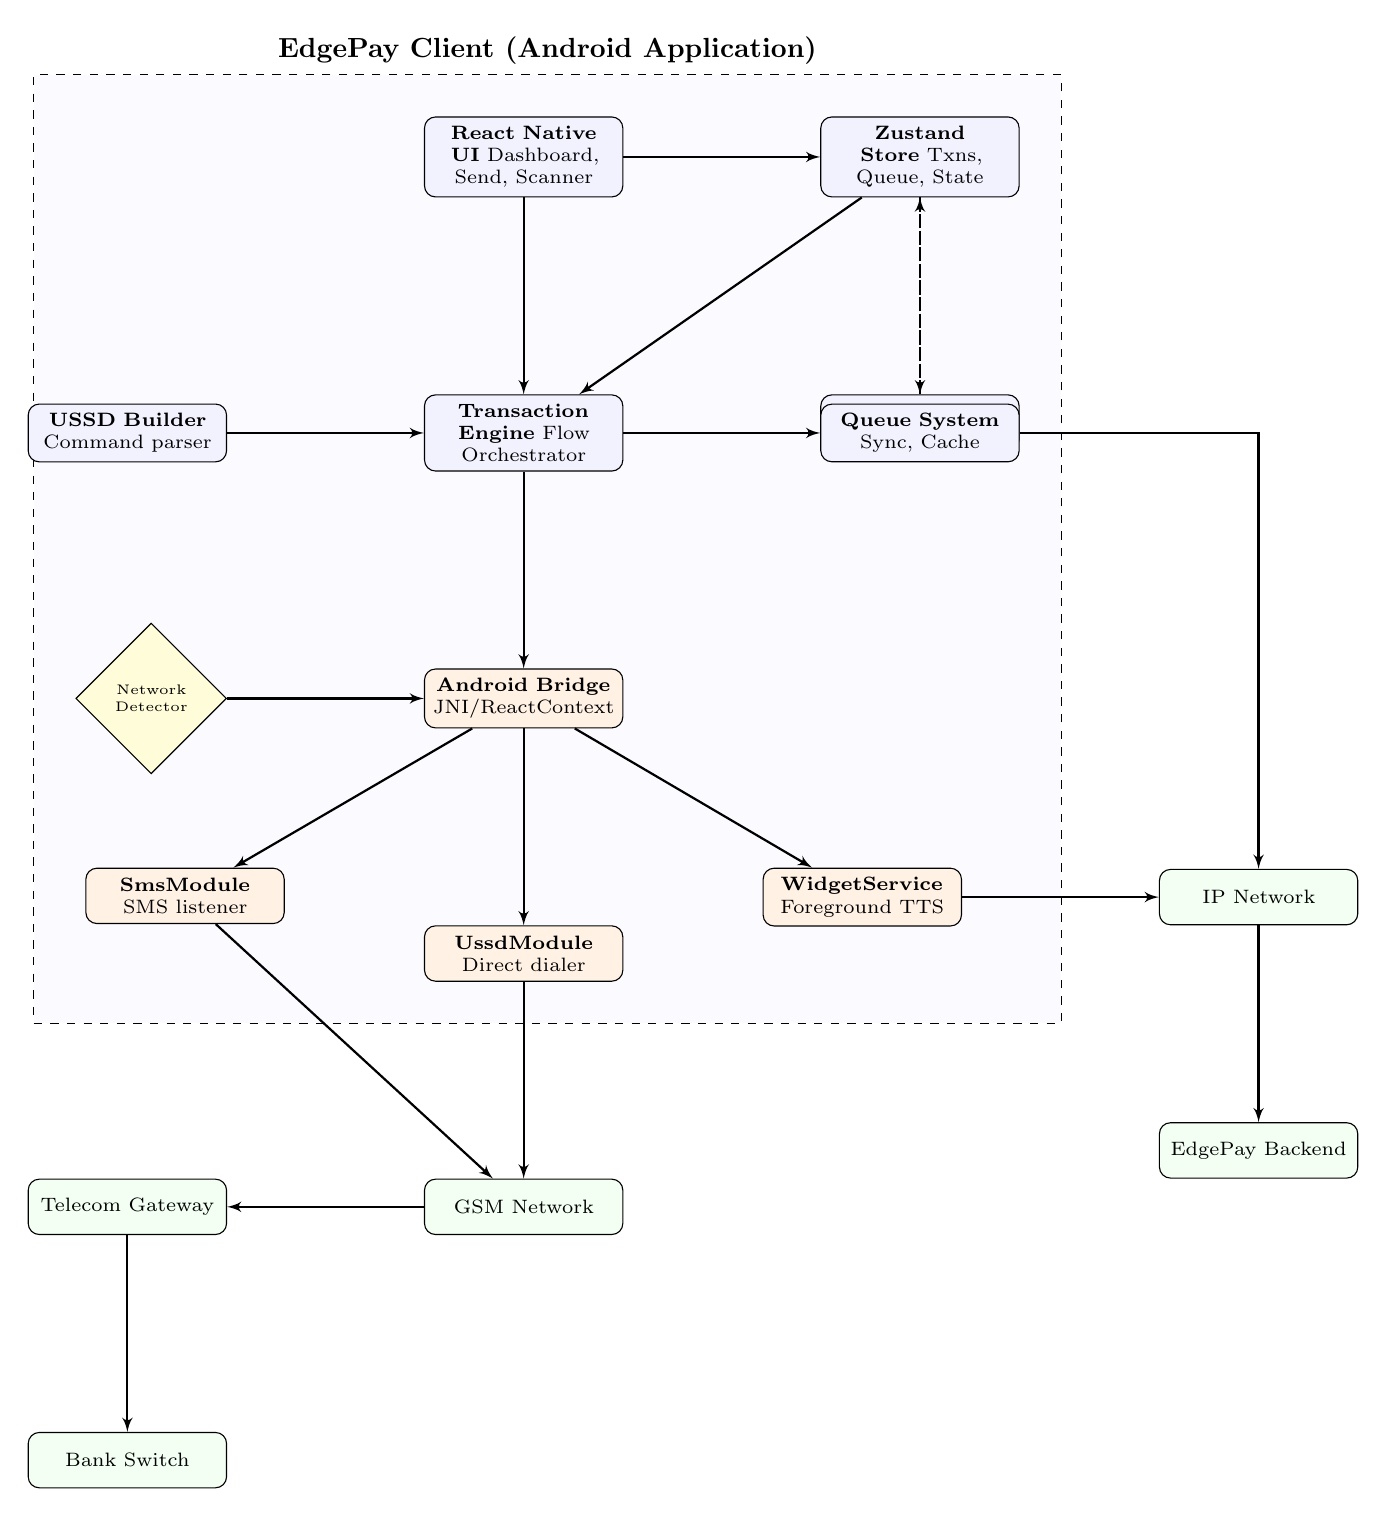
\begin{tikzpicture}[auto, node distance=2.0cm, >=latex']
    % Draw blocks
    \node (ui) [block] {\textbf{React Native UI} Dashboard, Send, Scanner};
    \node (store) [block, right=of ui] {\textbf{Zustand Store} Txns, Queue, State};
    \node (storage) [block, below=of store] {\textbf{AsyncStorage} Local serialization};
    
    \node (engine) [block, below=of ui] {\textbf{Transaction Engine} Flow Orchestrator};
    \node (queue) [block, right=of engine] {\textbf{Queue System} Sync, Cache};
    \node (ussdb) [block, left=of engine] {\textbf{USSD Builder} Command parser};
    
    \node (bridge) [native, below=of engine] {\textbf{Android Bridge} JNI/ReactContext};
    
    \node (sms_mod) [native, below left=of bridge] {\textbf{SmsModule} SMS listener};
    \node (ussd_mod) [native, below=of bridge] {\textbf{UssdModule} Direct dialer};
    \node (sound_mod) [native, below right=of bridge] {\textbf{WidgetService} Foreground TTS};
    
    \node (detector) [net, left=of bridge] {Network Detector};
    
    % External layers
    \node (gsm) [ext, below=of ussd_mod] {GSM Network};
    \node (telco) [ext, left=of gsm] {Telecom Gateway};
    \node (bank) [ext, below=of telco] {Bank Switch};
    
    \node (internet) [ext, right=of sound_mod] {IP Network};
    \node (backend) [ext, below=of internet] {EdgePay Backend};

    % Links
    \draw [arrow] (ui) -- (store);
    \draw [arrow, dashed] (store) -- (storage);
    \draw [arrow, dashed] (storage) -- (store);
    
    \draw [arrow] (ui) -- (engine);
    \draw [arrow] (store) -- (engine);
    \draw [arrow] (ussdb) -- (engine);
    \draw [arrow] (engine) -- (queue);
    
    \draw [arrow] (engine) -- (bridge);
    \draw [arrow] (bridge) -- (sms_mod);
    \draw [arrow] (bridge) -- (ussd_mod);
    \draw [arrow] (bridge) -- (sound_mod);
    \draw [arrow] (detector) -- (bridge);
    
    \draw [arrow] (ussd_mod) -- (gsm);
    \draw [arrow] (sms_mod) -- (gsm);
    \draw [arrow] (gsm) -- (telco);
    \draw [arrow] (telco) -- (bank);
    
    \draw [arrow] (sound_mod) -- (internet);
    \draw [arrow] (queue) -| (internet);
    \draw [arrow] (internet) -- (backend);
    
    % Background box
    \begin{scope}[on background layer]
        \node (client_box) [draw, dashed, fill=blue!2, inner sep=15pt, label=above:\textbf{EdgePay Client (Android Application)}, fit=(ui) (store) (storage) (engine) (queue) (bridge) (sms_mod) (ussd_mod) (sound_mod) (detector)] {};
    \end{scope}
\end{tikzpicture}
\caption{EdgePay Decoupled Component Architecture Diagram.}
\label{fig:full_arch}
\end{figure*}

\subsection{High-Level Application Loop}
As diagrammed in Fig.~\ref{fig:full_arch}, the application logic runs primarily offline. The Zustand store serves as the central data hub. The system's components function as follows:
\begin{enumerate}
    \item \textbf{Transaction Engine (\texttt{TransactionEngine.ts})}: Validates recipient and amount boundaries, compiles dialing strings via the \texttt{USSDBuilder}, and routes actions to the platform-specific bridges.
    \item \textbf{USSD Builder}: Formats inputs to match GSM shortcode protocols, sanitizing recipients' identifiers (phone numbers or UPI IDs) into standardized sequences.
    \item \textbf{Queue System (\texttt{QueueSystem.ts})}: Handles offline storage. Transactions that fail to reconcile immediately due to network delays are cached to local storage and marked for subsequent synchronization.
    \item \textbf{Network Detector (\texttt{NetworkDetector.ts})}: Combines Android system notifications with periodic lightweight HTTP checks (pinging \texttt{clients3.google.com/generate\_204}) to transition the system state dynamically between \texttt{ONLINE} and \texttt{GSM} modes.
\end{enumerate}

\subsection{UI Navigation Flow Architecture}
To guide the user through this process, the application implements a structured navigation architecture (illustrated in Fig.~\ref{fig:nav_flow}).

\begin{figure}[htbp]
\centering
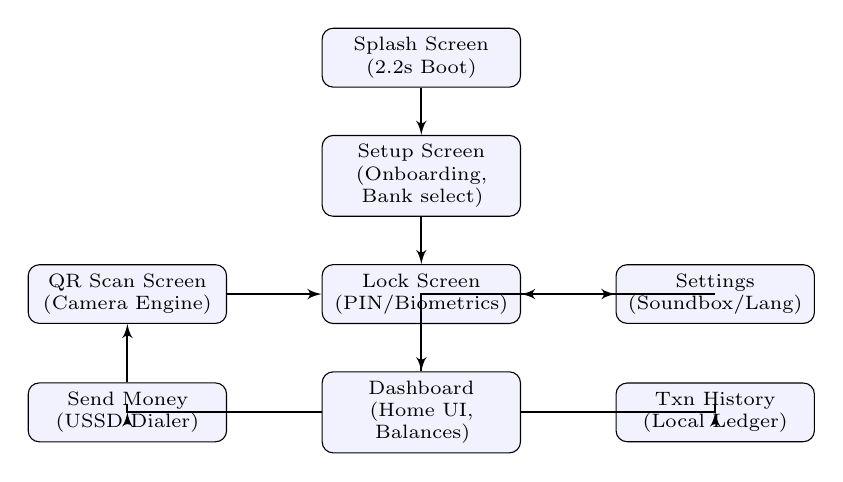
\begin{tikzpicture}[auto, node distance=1.5cm, >=latex']
    \node (splash) [block] {Splash Screen\\(2.2s Boot)};
    \node (setup) [block, below=0.6cm of splash] {Setup Screen\\(Onboarding, Bank select)};
    \node (lock) [block, below=0.6cm of setup] {Lock Screen\\(PIN/Biometrics)};
    \node (dash) [block, below=0.6cm of lock] {Dashboard\\(Home UI, Balances)};
    
    \node (send) [block, left=1.2cm of dash] {Send Money\\(USSD Dialer)};
    \node (scan) [block, left=1.2cm of lock] {QR Scan Screen\\(Camera Engine)};
    \node (history) [block, right=1.2cm of dash] {Txn History\\(Local Ledger)};
    \node (settings) [block, right=1.2cm of lock] {Settings\\(Soundbox/Lang)};
    
    \draw [arrow] (splash) -- (setup);
    \draw [arrow] (setup) -- (lock);
    \draw [arrow] (lock) -- (dash);
    
    \draw [arrow] (dash) -| (send);
    \draw [arrow] (send) -- (scan);
    \draw [arrow] (scan) -- (lock);
    \draw [arrow] (dash) -| (history);
    \draw [arrow] (dash) |- (settings);
    \draw [arrow] (settings) |- (lock);
\end{tikzpicture}
\caption{EdgePay User Journey and Navigation Flow.}
\label{fig:nav_flow}
\end{figure}

\begin{figure*}[htbp]
\centering
\begin{tabular}{ccc}
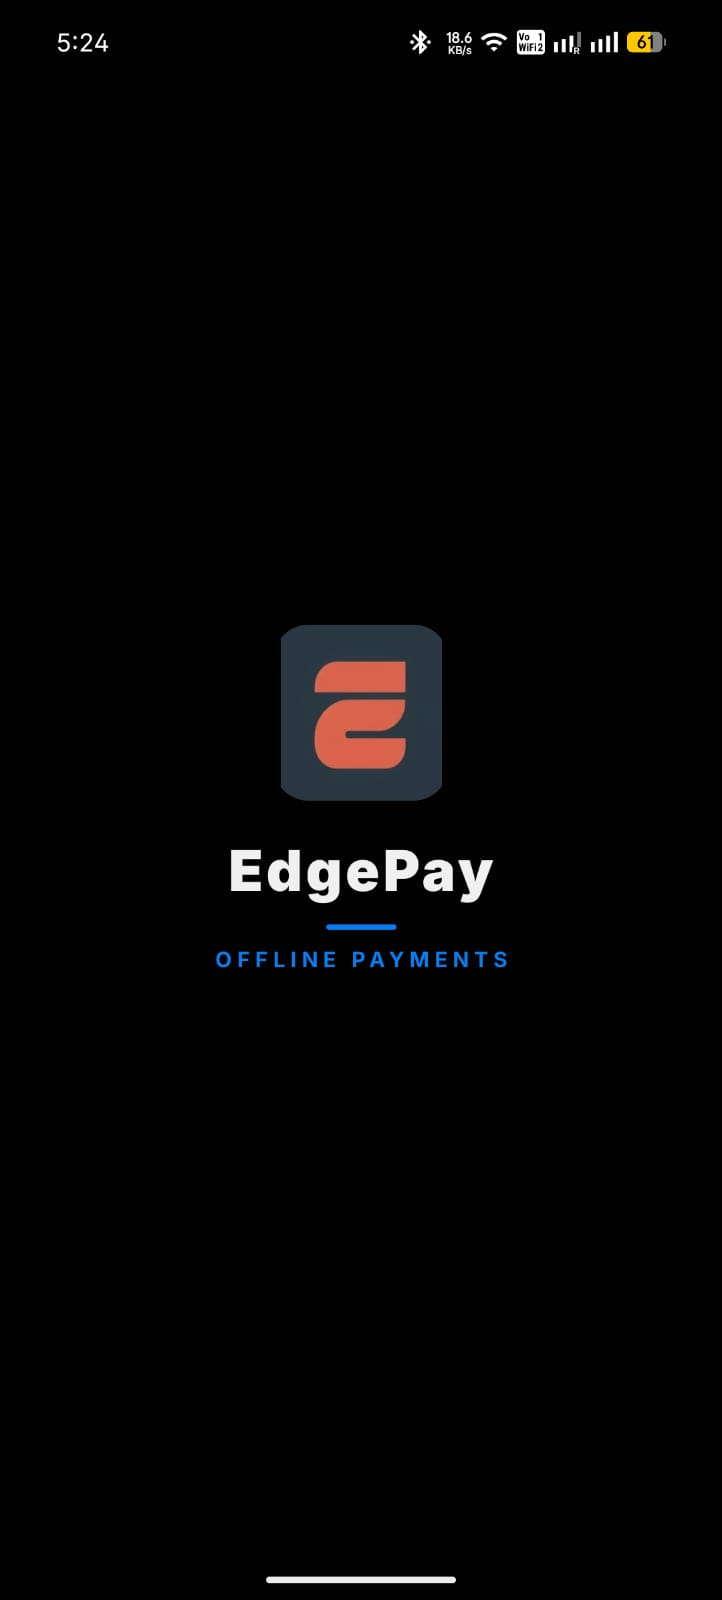
\includegraphics[width=0.28\textwidth]{img/screenshot_1.jpg} &
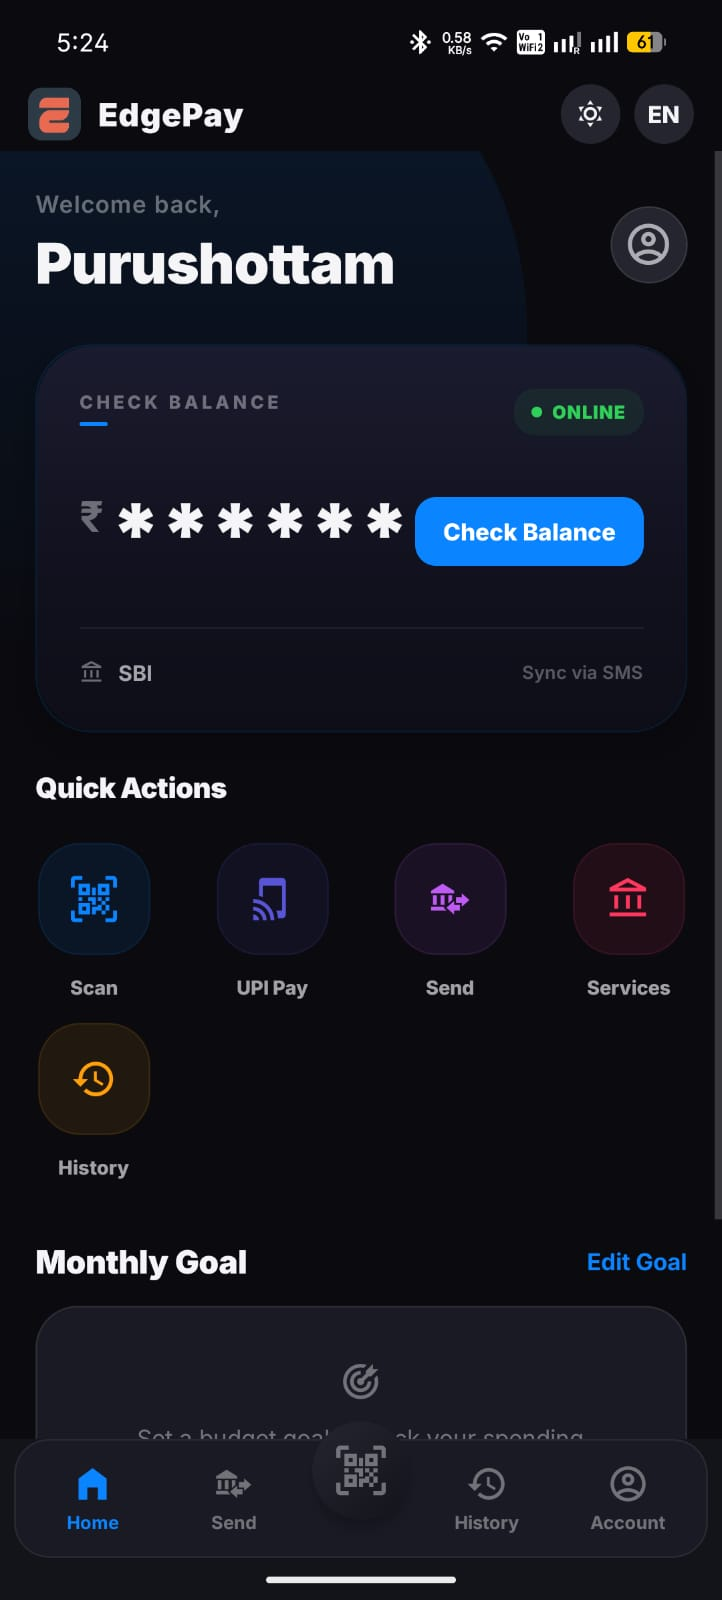
\includegraphics[width=0.28\textwidth]{img/screenshot_2.jpg} &
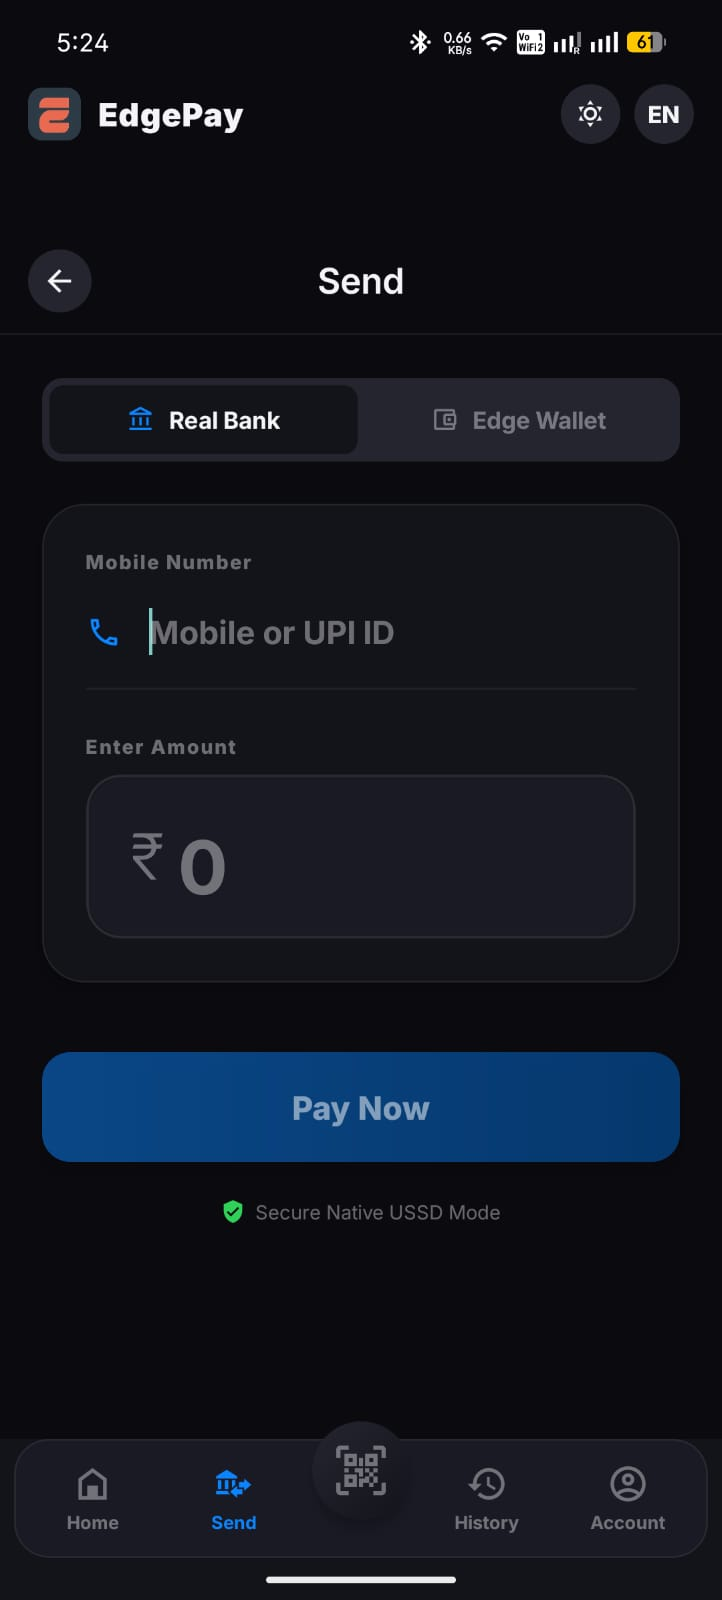
\includegraphics[width=0.28\textwidth]{img/screenshot_3.jpg} \\
(a) Setup / Onboarding Flow & (b) Security Lock Access & (c) Dashboard View \\ [1em]
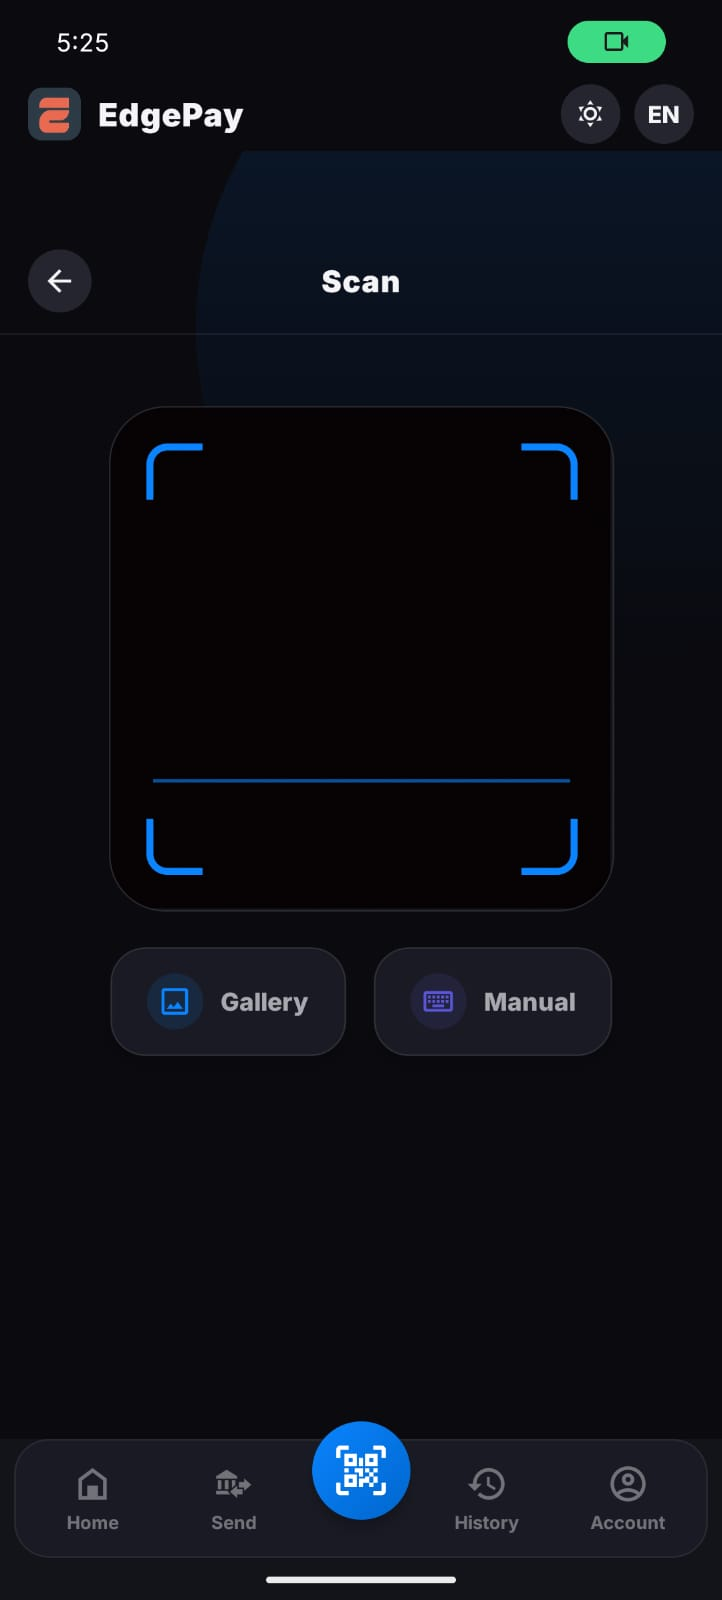
\includegraphics[width=0.28\textwidth]{img/screenshot_4.jpg} &
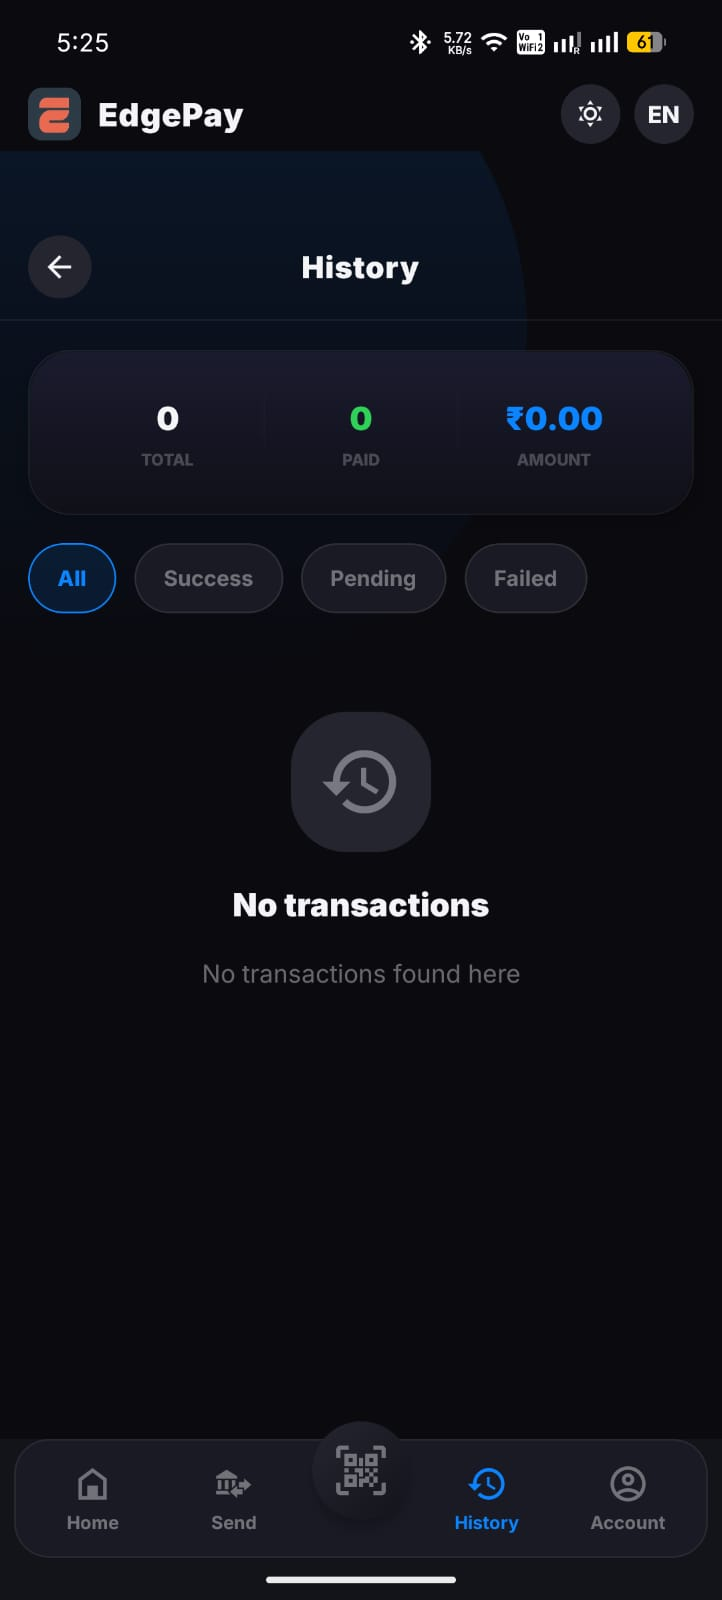
\includegraphics[width=0.28\textwidth]{img/screenshot_5.jpg} &
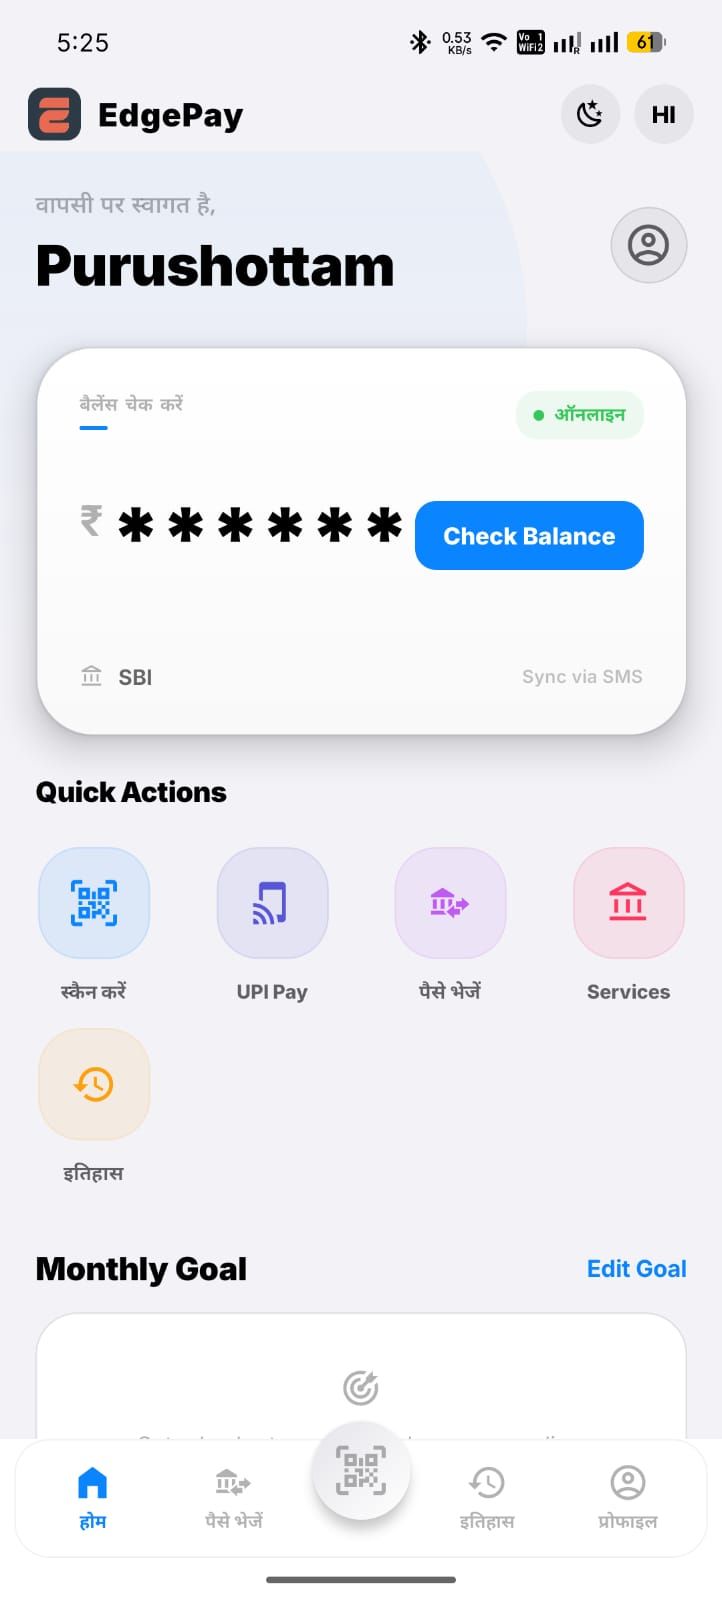
\includegraphics[width=0.28\textwidth]{img/screenshot_6.jpg} \\
(d) Offline Transaction Setup & (e) Live USSD Dialer Process & (f) Dynamic Voice Box Notification
\end{tabular}
\caption{EdgePay Real-World Android Application Screenshots and User Interface Workflow.}
\label{fig:screenshots}
\end{figure*}

\section{Protocol Interface, Verification, and Reconciliation}
To manage bank transactions over cellular channels, EdgePay implements custom string formatting and regex-based SMS parsing.

\subsection{USSD Dialing Syntax Construction}
The \texttt{USSDBuilder} translates recipient credentials and transfer amounts into standardized command sequences:
\begin{itemize}
    \item \textbf{Standard Phone Transfer}: \texttt{*99*1*1*\{sanitized\_phone\}*\{amount\}\#}
    \item \textbf{UPI ID / VPA Transfer}: \texttt{*99*1*3*\{sanitized\_vpa\}*\{amount\}\#}
\end{itemize}

During initial development, appending a terminal remark index (like \texttt{*1\#}) caused errors on certain bank networks. The bank switches sometimes parsed this extra digit as the first character of the user's UPI PIN, returning a ``UPI PIN Length is Incorrect'' error. Leaving the string open with a terminating \texttt{\#} allows the carrier's gateway to request remarks or PINs directly through native prompt overlays.

\subsection{Regex-Based SMS Parsing Engine}
Reconciling offline transactions relies on parsing incoming bank notification SMS messages. EdgePay uses regex patterns to extract transaction status, amounts, and source information:

\begin{lstlisting}[caption={Core regular expressions for extracting values from bank notifications.}]
// Pattern for extracting transaction amount
const AMOUNT_REGEX = /(?:RS|INR|[\u20B9])\.?\s*([0-9]+\.?[0-9]*)/i;

// Pattern for extracting reference number
const REF_REGEX = /(?:REF|TXN|UTR|IMPS)[\s.:#]*([A-Z0-9]{8,20})/i;

// Pattern for HDFC Bank balance confirmations
const HDFC_BAL_REGEX = /Avail Bal\s*[:.-]?\s*(?:RS|[\u20B9])\s*([0-9]+\.?[0-9]*)/i;
\end{lstlisting}

EdgePay checks incoming sender headers against verified bank prefixes (such as \texttt{SBIPSG}, \texttt{HDFCBK}, \texttt{ICICIB}) to prevent spoofing. If a message contains debit keywords (e.g., \texttt{debited}, \texttt{sent Rs}, \texttt{transferred}), the transaction engine reconciles the transaction locally.

\section{Offline Dual-Phase Verification Flow}
Because Android pauses third-party background threads during active USSD dialogs, standard broadcast receivers can miss incoming notifications. To handle this, EdgePay uses a dual-phase verification flow.

\subsection{Phase Execution Flow}
The transaction engine coordinates these steps to ensure reliable payment confirmations:
\begin{enumerate}
    \item The client initiates a transaction, generating a unique ID (e.g., \texttt{EP1782845...}).
    \item The app issues a system-level dial intent via \texttt{UssdModule.kt}.
    \item The user enters their UPI PIN via the native carrier dialog.
    \item Once the dialog closes, the app starts a 120-second tracking timer.
    \item \textbf{Real-Time Listener}: The registered native receiver monitors incoming broadcast intents.
    \item \textbf{Inbox Polling Fallback}: Concurrently, a background worker queries the local SMS inbox provider every 3 seconds to capture messages that may have arrived while the dialog overlay was active.
    \item If a matching transaction is found, the app updates the local store status to \texttt{SUCCESS} and plays an offline voice confirmation.
\end{enumerate}

\subsection{Verification Algorithm Logic}
The transactional check logic is structured as follows:

\begin{algorithmic}[1]
\REQUIRE $amount > 0$, $receiver \neq \emptyset$, $timeout = 120\text{s}$
\ENSURE TransactionStatus $\in \{\text{SUCCESS}, \text{FAILED}\}$
\STATE $txn \leftarrow \text{CreateTransaction}(amount, receiver)$
\STATE $dialString \leftarrow \text{USSDBuilder.buildUssdCommand}(receiver, amount)$
\STATE $\text{UssdModule.dialUssdCode}(dialString)$
\STATE $startTime \leftarrow \text{GetCurrentTime}()$
\STATE $resolved \leftarrow \text{FALSE}$
\WHILE{$\text{GetCurrentTime}() - startTime < timeout$ \AND \NOT $resolved$}
    \STATE $smsList \leftarrow \text{SmsModule.readRecentSms}(15)$
    \FORALL{$sms$ \textbf{in} $smsList$}
        \IF{$sms.timestamp \ge startTime - 5000$}
            \IF{$\text{isBankSms}(sms.sender)$ \AND $\text{parseSmsForTransaction}(sms) == \text{SUCCESS}$}
                \STATE $\text{UpdateTxnStatus}(txn.id, \text{SUCCESS})$
                \STATE $\text{PaymentSoundbox.announce}(txn)$
                \STATE $resolved \leftarrow \text{TRUE}$
                \STATE \textbf{return} SUCCESS
            \ENDIF
        \ENDIF
    \ENDFOR
    \STATE $\text{Sleep}(3000\text{ms})$
\ENDWHILE
\STATE $\text{UpdateTxnStatus}(txn.id, \text{FAILED})$
\STATE $\text{QueueSystem.enqueue}(txn)$
\STATE \textbf{return} FAILED
\end{algorithmic}

\section{Security Architecture \& Cryptographic Controls}
Operating offline means EdgePay cannot rely on standard remote HTTPS handshakes to secure transaction endpoints. Instead, the application implements local security controls:

\subsection{Storage Masking and Dashboard Security}
To defend against unauthorized screen viewing, the app masks financial data by default. The primary balance indicator displays a masked value (\texttt{₹ ******}) until the user passes a biometric authentication check.

\subsection{PIN Management and Memory Lifecycle}
EdgePay handles user authentication pins securely:
\begin{itemize}
    \item \textbf{Cryptographic Hashing}: The user's onboarding PIN is processed locally using key-derivation algorithms (PBKDF2) and stored in securely encrypted preferences.
    \item \textbf{Memory Clean Lifecycle}: To prevent memory harvesting via runtime debuggers, any clear-text values collected from the PIN input components are immediately zeroed out after authentication check loops:
\begin{lstlisting}[caption={Secure zero-fill operation in native memory.}]
// Zero out sensitive variables from memory arrays
fun clearPinArray(pin: CharArray) {
    for (i in pin.indices) {
        pin[i] = '\u0000'
    }
}
\end{lstlisting}
\end{itemize}

\subsection{Verification of Broadcast Authenticity}
To prevent spoofing via fake SMS, the native listener matches incoming messages against a verified list of shortcodes (e.g., matching the \texttt{AD-} country code and bank signature format). Messages originating from standard 10-digit mobile numbers are ignored for transaction confirmations.

\section{The Payment Soundbox \& Background Services}
For merchants in busy market environments, checking screens for payment confirmations is inconvenient. EdgePay includes a built-in voice confirmation feature (the ``Soundbox'').

\subsection{Foreground Service Architecture}
To prevent the OS from closing the listener in the background, EdgePay uses an Android Foreground Service (\texttt{PaymentWidgetService}). This service runs with an active status notification, maintaining memory priority even under low-system resource conditions.

\subsection{Offline TTS Pipeline}
The audio alerts operate locally without internet access:
\begin{enumerate}
    \item The service receives an event notification containing transaction details.
    \item The text engine processes the transaction details into localized announcement scripts.
    \item The system checks the local language settings (supporting Hindi, Marathi, Urdu, Bengali, Kannada, Odia, Punjabi, and English).
    \item The text-to-speech engine speaks the formatted confirmation string (e.g., \textit{``EdgePay. Two hundred rupees received from Jane Doe.''})
\end{enumerate}

\section{Reconciliation and Queue Synchronization}
Transactions that fail to receive immediate confirmation SMS (due to signal outages) are stored locally in a persistent retry queue using AsyncStorage.

\begin{lstlisting}[caption={Structure of a queued transaction awaiting sync.}]
{
  "id": "EPK9V1M3X8",
  "amount": 250.00,
  "receiver": "jane@okhdfc",
  "receiverName": "Jane Doe",
  "method": "USSD",
  "status": "QUEUED",
  "timestamp": 1782845300000,
  "retryCount": 1
}
\end{lstlisting}

When the \texttt{NetworkDetector} flags that internet connectivity has been restored, the app triggers a synchronization process:
\begin{enumerate}
    \item The queue module loads pending items from storage.
    \item The app sends the transaction array to the Express API backend: \texttt{POST /api/transactions/sync}.
    \item The backend deduplicates the incoming records by transaction ID.
    \item The backend writes new transactions atomically to the database file:
\begin{lstlisting}[caption={Atomic file write pattern in the backend sync server.}]
function saveJson(filePath, data) {
    const tmpFile = filePath + '.tmp';
    fs.writeFileSync(tmpFile, JSON.stringify(data, null, 2), 'utf-8');
    fs.renameSync(tmpFile, filePath); // Atomic rename preserves file integrity
}
\end{lstlisting}
    \item The app clears reconciled items from the local queue.
\end{enumerate}

\section{Real-World Deployment \& Scaling Roadmap}
Deploying an offline-first financial application requires a phased rollout to handle telecom network variations and meet regulatory compliance standards.

\begin{table*}[htbp]
\caption{EdgePay Project Roadmap Phases and Deliverables}
\label{tab:roadmap_milestones}
\centering
\scriptsize
\begin{tabular}{lp{2.5cm}p{9.5cm}}
\toprule
\textbf{Milestone Phase} & \textbf{Timeline} & \textbf{Key Action Items \& Deliverables} \\
\midrule
Phase 1: Stabilization & Months 0 - 3 & \begin{itemize} \item Standardize SMS parser regex patterns. \item Test compatibility with custom Android ROMs. \item Optimize battery usage of background service. \end{itemize} \\
\midrule
Phase 2: Regulatory Pilot & Months 3 - 6 & \begin{itemize} \item Conduct OWASP security and penetration audits. \item Secure NPCI sandboxed API access. \item Launch a pilot with 500 merchants in low-connectivity areas. \end{itemize} \\
\midrule
Phase 3: Scale \& Hardware & Months 6 - 12 & \begin{itemize} \item Launch public app on Google Play Store. \item Develop an ESP32-based hardware soundbox companion. \item Integrate local credit scoring based on transaction history. \end{itemize} \\
\bottomrule
\end{tabular}
\end{table*}

\subsection{Phase 1: Native Engine Stabilization (0 - 3 Months)}
The initial phase addresses compatibility challenges across different Android versions. Some custom Android distributions (e.g., Xiaomi's MIUI, Oppo's ColorOS) restrict background services and auto-start behaviors. This phase focuses on developing setup tutorials and system prompt routines to guide users in whitelist settings. We will also expand the regex dictionary to support regional rural banks in India.

\subsection{Phase 2: Regulatory Compliance \& Pilot Trials (3 - 6 Months)}
Because EdgePay handles financial transactional data, meeting local regulatory requirements is essential. This phase focuses on:
\begin{itemize}
    \item \textbf{Regulatory Compliance}: Partnering with sponsor banks to access the NPCI *99\# gateway gateway.
    \item \textbf{Field Trials}: Testing application performance in rural markets with poor telecom coverage to evaluate SMS parsing accuracy.
\end{itemize}

\subsection{Phase 3: Public Release and Hardware Companions (6 - 12 Months)}
After stabilization, the application will be released on the Google Play Store, targeting low-resource smartphones. In parallel, we will develop a physical soundbox companion utilizing low-cost ESP32 microcontrollers. 

This desktop soundbox will connect to the merchant's phone via Bluetooth, letting them receive audio confirmations without requiring constant internet access or expensive dedicated terminal devices.

\begin{figure}[htbp]
\centering
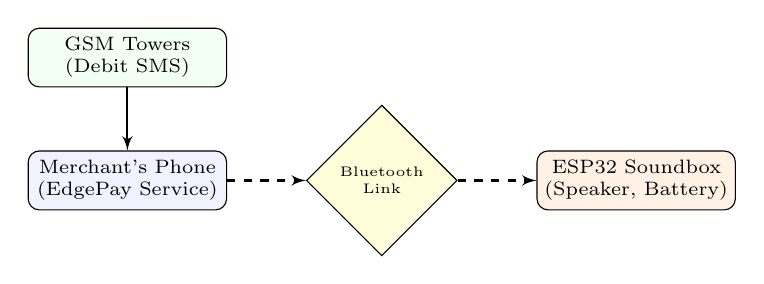
\begin{tikzpicture}[node distance=1.5cm, auto, >=latex']
    \node (phone) [block] {Merchant's Phone\\(EdgePay Service)};
    \node (bt) [net, right=1.0cm of phone] {Bluetooth\\Link};
    \node (soundbox) [block, right=1.0cm of bt, fill=orange!10] {ESP32 Soundbox\\(Speaker, Battery)};
    
    \node (telecom) [ext, above=0.8cm of phone] {GSM Towers\\(Debit SMS)};
    
    \draw [arrow] (telecom) -- (phone);
    \draw [arrow, dashed] (phone) -- (bt);
    \draw [arrow, dashed] (bt) -- (soundbox);
\end{tikzpicture}
\caption{ESP32-based Merchant Desktop Soundbox Architecture.}
\label{fig:soundbox_arch}
\end{figure}

\section{Conclusion}
EdgePay demonstrates how wrapping legacy communication channels in a modern smartphone application can improve digital payment accessibility. By combining GSM networks and the NPCI *99\# gateway with local SMS parsing and offline speech synthesis, EdgePay reduces transaction friction in low-connectivity areas. The platform offers a reliable alternative for digital payments in remote environments, supporting broader financial inclusion goals.

\section*{Availability \& Repository Details}
The codebase, technical specifications, and development assets are available in the project repository: \url{https://github.com/yash-hackathon-email/edgepay.git}.

\begin{thebibliography}{00}
\bibitem{b1} NPCI, ``*99\# National Unified USSD Platform (NUUP) Technical Guide,'' National Payments Corporation of India, Mumbai, 2021.
\bibitem{b2} GSMA, ``Financial Inclusion in Emerging Markets: The Role of Offline Mobile Money Protocols,'' Global System for Mobile Communications Association, London, 2022.
\bibitem{b3} A. Kumar and S. Sen, ``Resilient digital payment networks for remote regions using USSD and SMS fallback bridges,'' in \textit{IEEE Transactions on Consumer Electronics}, vol. 68, no. 3, pp. 214--221, Aug. 2022.
\end{thebibliography}

\end{document}
